\documentclass[11pt, a4paper]{article}

\usepackage{amsmath}
\usepackage{amsfonts} %Matheschriften
\usepackage{amssymb} %Mathesymbole
%\usepackage{mathptmx} % Einstellung für Schriften und Sonderzeichen in mathematischen Umgebungen
                        % ändert SChriftfont
\usepackage{wasysym} % Stellt diverse Sonderzeichen bereit
\usepackage{siunitx}
\usepackage{float}
\usepackage{microtype}
\usepackage{graphicx}
\usepackage{hyperref}
\usepackage{xcolor}
\usepackage[section]{placeins}
% allows for temporary adjustment of side margins
\usepackage{changepage}
\usepackage{rotating}
\usepackage{physics}

\usepackage[ngerman]{babel}
\addto\captionsngerman{%
 \renewcommand{\abstractname}{Einleitung}}


\title{Versuch 3: Beugung und Brechung}
\author{Team 4-11: Jascha Fricker, Benedict Brouwer}

\begin{document}
    \maketitle

    \tableofcontents

    \newpage

    \section{Theorie}
    \FloatBarrier
    In diesem Versuch wurde mit einem Einfachspalt, einem Gitter und einem Prisma Phänomene der Beugung und Brechung untersucht. 

    \subsection{Beugung am Einfachspalt}
    Bei bestrahlung eines Einfachspalts (mit Spaltbreite $d$) mit kohärentem Licht der Wellenlänge $\lambda$ entsteht auf dem Schirm mit Abstand $l$ ein Beugungsbild bestehend aus Minima und Maxima mit Abstand $s$ zum Maxima nullter Ordnung. Dessen Position kann mit folgenden Fromeln berechnet werden:
    \begin{align}
        \frac{n * \lambda}{d} = sin{\alpha} \approx \tan{\alpha} = \frac{s_{Minima}}{l} \label{eq:einfachspalt} \\
        \frac{(n + \frac{1}{2})* \lambda}{d} = sin{\alpha} \approx \tan{\alpha} = \frac{s_{Maxima}}{l} 
    \end{align}
    \subsection{Beugung am Gitter}
    Wird ein Gitter mit Gitterkonstante $a$ bestrahlt so entsteht auf dem Schirm ein charakteristisches Beugungsbilt mit Hauptmaxima n-ter Ordnung mit Entfernung $s$ zum Mittelpunkt. Deren Position Kann Berechnet werden mit:
    \begin{align}
        \frac{n * \lambda}{a} = sin{\alpha} \approx \tan{\alpha} = \frac{s_{Maxima}}{l} \label{eq:Gitter} \\
        
    \end{align}
    \section{Ergebnisse}
    \subsection{Einfachspalt}
    In diesem Versuchsteil wurde mit einem Laser der Wellenlänge $\lambda = 532(1)\si{\nano\meter}$ ein Einfachspalt bestrahlt und dessen Beugungsbild untersucht.
    Dazu wurde bei drei unterschiedlichen Schirmabständen der Abstand der Minima der Jeweiligen Ordnung zueinander gemessen. Bei der Auswertung wurde die Kleinwinkelnäherung angewerndet, da im Extremalfall $\arctan(\frac{s}{l}) = 1,1457°$ und $\arcsin(\frac{s}{l}) = 1,1459°$
    was einer Abweichung von $0,017\percent$ entspricht. Die Messergebnisse wurden in Graph \ref{fig:einzelspalt} geplottet und mit einer Ausgleichsgerade $a \cdot x + b$ mit den Parametern $a = 3,64(13) \cdot 10^{-3}$ und $b= -1,05 \cdot 10^{-4}$ gefittet.
    Mit disen Parameter lässt sich aus Formel \ref{eq:einfachspalt} und mithilfe der gaußschen Fehlerfortpflanzung die Spaltbreite berechnen zu $d= 146(5) \cdot 10^{-3}$. Die Fehlerbalken wurden mit dem Analogenfehler eines Metermaßes und Fehlerfortpflanzung berechent.
    

    
    \begin{figure}
        \centering
        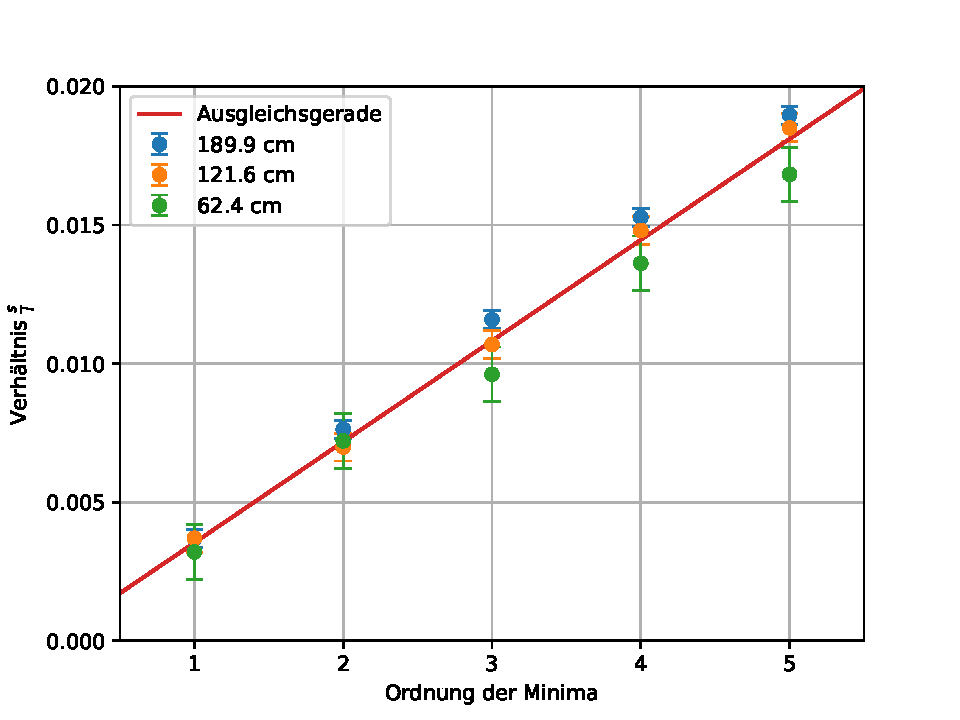
\includegraphics[width=0.8\textwidth]{./plots/einzelspalt.pdf}
        \caption{Messergebnisse des Einzelspalts}
        \label{fig:einzelspalt}
    \end{figure}
    \subsection{Berechnung der Wellenlängen einer Hg Lampe}
    Um die charakteristischen Wellenlängen einer Quksilberdampf-Lampe zu bestimmen wird in diesem Versuchsteil deren Licht auf ein Gitter mit einer Gitterkonstante von $a=10.00(02)\cdot \si{\micro\metre}$ gerichtet.
    Anschließend wurde bei drei unterschiedlichen Abständen der Abstand der Maxima gleicher Ordnung zueinander gemessen für drei der Charakteristischen Wellenlängen. Hirbei kann nicht von der Kleinwinkelnäherung gebrauch gemacht werden, da im Extremalfall $\arctan(\frac{s}{l}) = 14.574°$ und $\arcsin(\frac{s}{l}) = 15,070°$
    was einer Abweichung von $2,14\percent$ entspricht. Daher wurde in der Auswertung $\sin(\arctan(\frac{s}{l}))$ gegen die Ordnung der Maxima für die Drei Wellenlängen wie in den Graphen \ref{fig:GitterBLAU}, \ref{fig:GitterGRÜN} und \ref{fig:GitterROT} zu sehen aufgetragen.
    Dabei fällt auf, das die Messwerte des Abstandes $26,15 \si{\centi\metre}$ eine hohe ungenauhigkeit aufweisen, was vermutlich an dem kleineren Abstand der Maxima bei dieser Länge liegt.
    mit 

    \begin{figure}
        \centering
        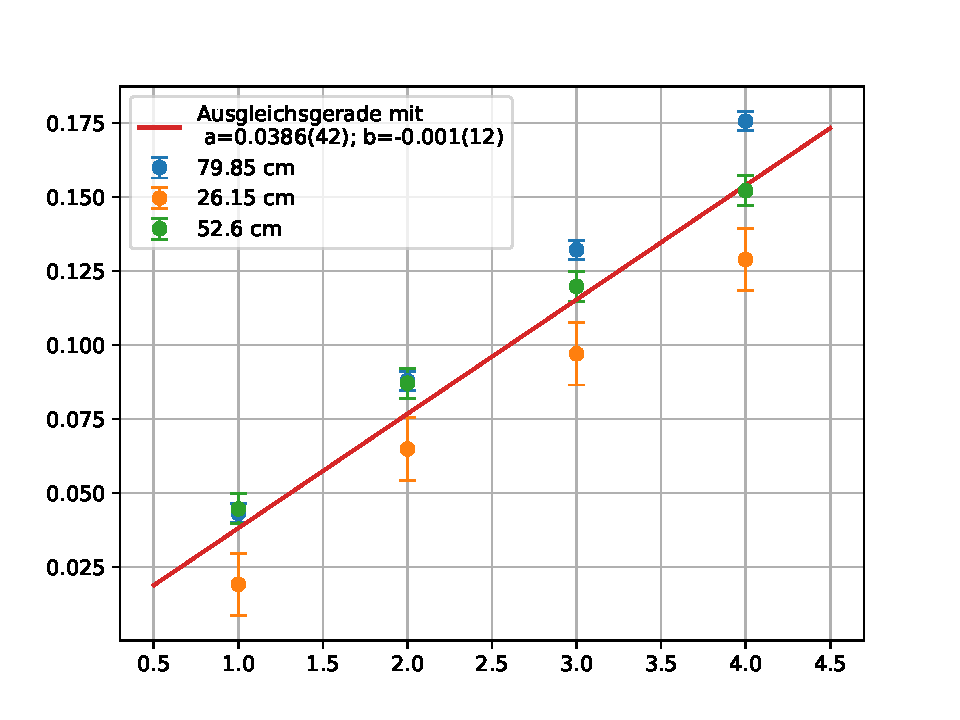
\includegraphics[width=0.8\textwidth]{./plots/Gitter_Blau.pdf}
        \caption{Messergebnisse am Gitter der blauen Wellenlänge}
        \label{fig:GitterBLAU}
    \end{figure}
    \begin{figure}
        \centering
        \includegraphics[width=0.8\textwidth]{./plots/Gitter_Grün.pdf}
        \caption{Messergebnisse am Gitter der grünen Wellenlänge}
        \label{fig:GitterGRÜN}
    \end{figure}
    \begin{figure}
        \centering
        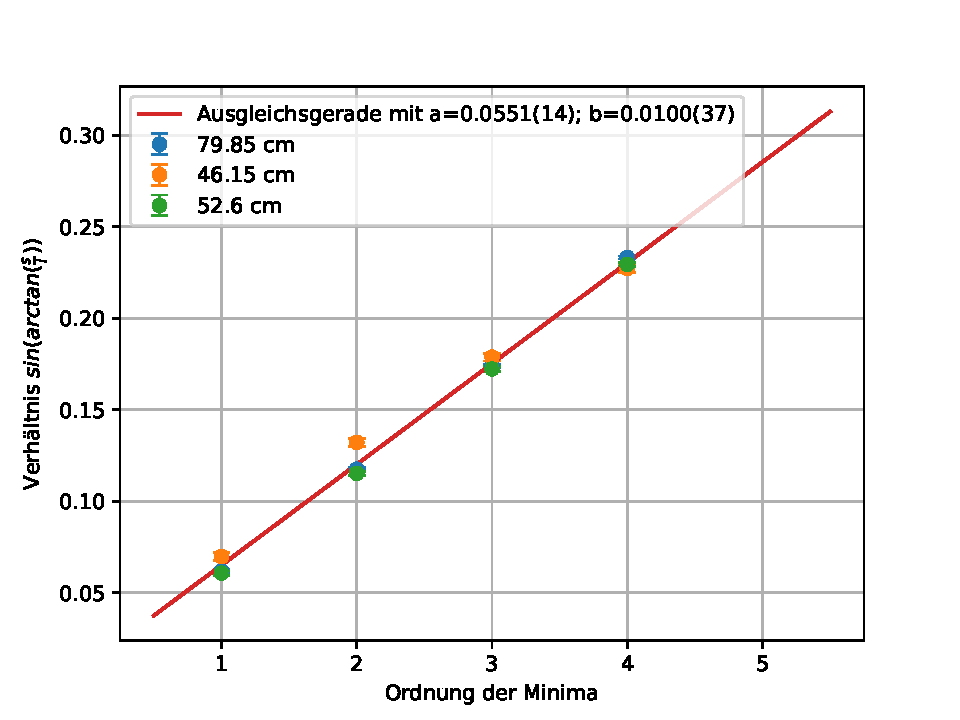
\includegraphics[width=0.8\textwidth]{./plots/Gitter_Rot.pdf}
        \caption{Messergebnisse am Gitter der roten Wellenlänge}
        \label{fig:GitterRot}
    \end{figure}



    \bibliographystyle{plain}
    \bibliography{literature}

\end{document}